% Drawing 148/02-12 -- folder 148, batch 02, archive page 32 (PDF page 33).
% Transcription: à droite, une colonne de croquis au crayon et à l'encre verte. En haut, dans une boucle au crayon : un pantalon (trois bouts), une sphère à quatre trous découpée par une croix en pointillé vert, une seconde sphère à quatre trous découpée de même, et un croquis biffé. Au-dessous, dans une autre boucle : une sphère à cinq trous découpée par des courbes en pointillé vert, puis deux sphères à cinq trous vues de face, leurs trous dessinés comme de petits cercles et un goulot. En bas, séparé par un trait : un grand bord de surface, ovale, marqué de points et de petits traits, d'où partent les contours de la surface.
% Kind: column of sketches: pants, spheres with four and five holes cut by dotted curves, a large boundary curve. Method 2 (redraw from the facsimile). Status: partial.
% Notes: Redrawn from the colour scan at 350 dpi, figure by figure, every coordinate read on gridded crops and the result overlaid on the page. Upper group: the pants with its three end ovals, three outline arcs and a pencil seam; a four-ended surface with its four end ovals, four outline arcs and the green dotted cross (one cut across, one down); a four-ended surface seen as a tetrahedron (one end oval, an oval at the right, two rings in front), with its outline, an inner edge, three green dotted cuts and a black dashed line; the hatched scribble to its right is a struck sketch and is not drawn. Lower group: the five-ended surface with its five end ovals, five outline arcs and five green dotted cuts, each between two neighbouring ends (one of them partly solid); two spheres, each with a neck at the top, two rings in front (on the left sphere both heavy, on the right sphere one heavy and one plain), a dashed ring behind (on the right sphere a second dashed outline at the right), the line joining the front rings, dashed pieces of the back line, and four pencil bands across. The two pencil loops around the groups and the pencil rule under them are drawn in pencil. Bottom: the oval rim, drawn through 24 points read on it, with its two heavy points where the contours leave, six more dots, six crossed marks (stars) and nine ticks or small marks, in the order of the page; three pencil contours of the surface leaving the rim. Still differs: the pencil bands of the two spheres and the pencil loops are simplified (drawn as single smooth curves); the end ovals are true ellipses; on the rim the distinction between a tick and a small mark is not kept. Redrawn 2026-11-12 (issue 128): to check again.
% Coordinates: 1 unit = 1 mm = 1/100 of the crop width, y downwards as on the crop (bbox in page fractions: [0.68, 0.065, 0.995, 0.545]).
% Redrawn by Claude (claude-fable-5-2), issue #128, 2026-11-12, from the colour scan at 350 dpi; not checked by a human; not compiled (no TeX in the session).
% Rights: reproduces part of the work -- behind RENDER_TRANSCRIPTS, never published by itself.
\documentclass[tikz,border=3pt]{standalone}
\usepackage{amsmath,amssymb}
\usetikzlibrary{patterns,arrows.meta}
\tikzset{pencil/.style={black!45}, struck/.style={black!35}, mpt/.style={circle,draw,inner sep=1.3pt}, pt/.style={circle,fill,inner sep=0.9pt}, opt/.style={circle,draw,fill=white,inner sep=1.1pt}, Rd/.style={red!75!black}, Gn/.style={green!45!black}, Br/.style={brown!70!black}, Bl/.style={blue!70!black}}
\begin{document}
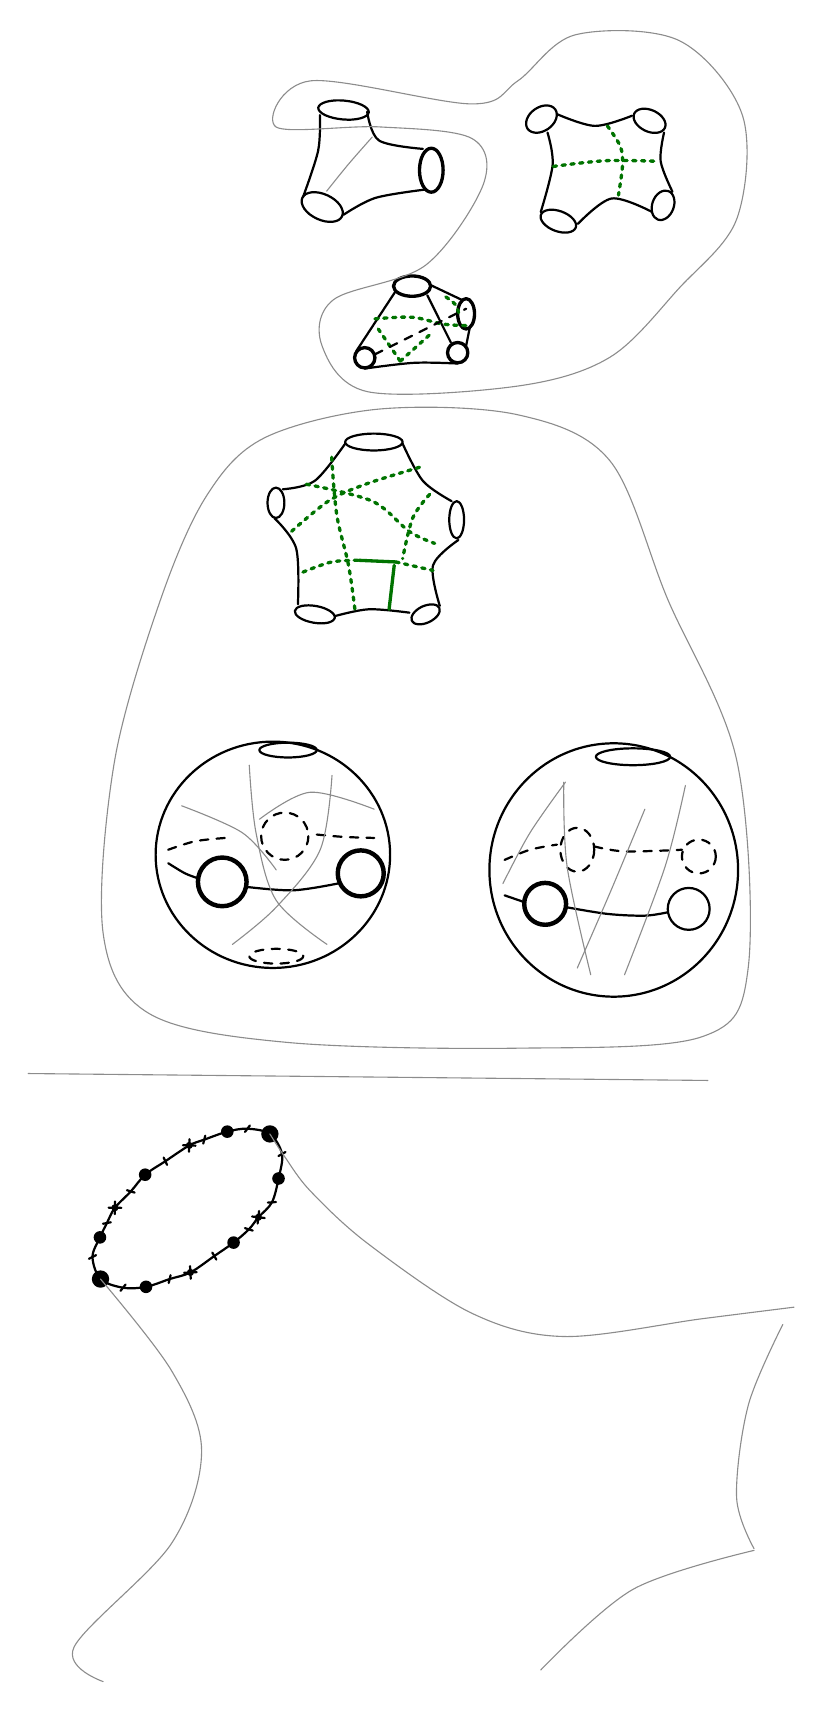
\begin{tikzpicture}[x=1mm,y=-1mm,line cap=round,line join=round,font=\small]
% pants
\draw[thick] plot[smooth cycle, tension=0.55] coordinates {(43.45,13.34) (43.16,13.77) (42.43,14.1) (41.37,14.27) (40.14,14.25) (38.92,14.05) (37.9,13.7) (37.24,13.25) (37.03,12.77) (37.32,12.34) (38.05,12.01) (39.11,11.84) (40.34,11.86) (41.56,12.06) (42.58,12.41) (43.24,12.86)};
\draw[very thick] (51.39,20.7) ellipse[x radius=1.5, y radius=2.79];
\draw[thick] plot[smooth cycle, tension=0.55] coordinates {(40.06,26.55) (39.61,27.03) (38.84,27.25) (37.87,27.19) (36.85,26.85) (35.93,26.29) (35.26,25.59) (34.94,24.85) (35.01,24.2) (35.47,23.72) (36.24,23.5) (37.21,23.56) (38.23,23.9) (39.14,24.46) (39.81,25.16) (40.14,25.9)};
\draw[thick] plot[smooth, tension=0.55] coordinates {(37.24,13.7) (37.02,18.21) (35.09,24.13)};
\draw[thick] plot[smooth, tension=0.55] coordinates {(43.24,13.27) (44.74,16.92) (50.32,17.99)};
\draw[thick] plot[smooth, tension=0.55] coordinates {(40.24,26.36) (44.32,24.21) (50.75,23.14)};
\draw[pencil] plot[smooth, tension=0.55] coordinates {(43.89,16.49) (40.88,19.92) (38.1,23.36)};
% four ends, green dotted cross
\draw[thick] plot[smooth cycle, tension=0.55] coordinates {(67.14,12.98) (67.33,13.54) (67.23,14.21) (66.85,14.87) (66.24,15.44) (65.5,15.81) (64.75,15.95) (64.09,15.81) (63.62,15.44) (63.43,14.87) (63.53,14.21) (63.91,13.54) (64.52,12.98) (65.26,12.6) (66.01,12.47) (66.67,12.6)};
\draw[thick] plot[smooth cycle, tension=0.55] coordinates {(81.05,15.33) (80.68,15.74) (80.07,15.94) (79.32,15.92) (78.53,15.67) (77.83,15.22) (77.32,14.66) (77.09,14.06) (77.16,13.51) (77.53,13.11) (78.14,12.9) (78.9,12.93) (79.69,13.18) (80.39,13.62) (80.89,14.18) (81.13,14.78)};
\draw[thick] plot[smooth cycle, tension=0.55] coordinates {(69.74,27.98) (69.4,28.38) (68.78,28.6) (67.97,28.6) (67.08,28.38) (66.27,27.98) (65.65,27.45) (65.31,26.89) (65.31,26.36) (65.64,25.96) (66.27,25.74) (67.08,25.74) (67.96,25.96) (68.78,26.36) (69.4,26.89) (69.74,27.45)};
\draw[thick] plot[smooth cycle, tension=0.55] coordinates {(82.11,25.62) (81.76,26.28) (81.27,26.77) (80.71,27.01) (80.16,26.97) (79.72,26.65) (79.44,26.1) (79.38,25.41) (79.53,24.68) (79.88,24.02) (80.38,23.54) (80.94,23.3) (81.48,23.34) (81.93,23.66) (82.2,24.2) (82.27,24.89)};
\draw[thick] plot[smooth, tension=0.55] coordinates {(67.31,13.56) (72.16,15.07) (76.88,13.78)};
\draw[thick] plot[smooth, tension=0.55] coordinates {(66.15,15.92) (66.8,20) (65.29,26.01)};
\draw[thick] plot[smooth, tension=0.55] coordinates {(70.01,27.51) (74.3,24.29) (79.45,26.01)};
\draw[thick] plot[smooth, tension=0.55] coordinates {(80.95,15.92) (80.52,19.57) (82.02,23.44)};
\draw[Gn,very thick,dotted] plot[smooth, tension=0.55] coordinates {(66.88,20.22) (73.53,19.49) (80.18,19.57)};
\draw[Gn,very thick,dotted] plot[smooth, tension=0.55] coordinates {(73.75,15.07) (75.38,17.64) (75.68,20) (75.16,23.86)};
% four ends seen as a tetrahedron
\draw[very thick] (48.95,35.42) ellipse[x radius=2.36, y radius=1.29];
\draw[very thick] (55.81,38.94) ellipse[x radius=1.07, y radius=1.93];
\draw[very thick] (42.94,44.52) circle[radius=1.29];
\draw[very thick] (54.74,43.87) circle[radius=1.29];
\draw[thick] (46.8,36.15) -- (41.87,43.66);
\draw[thick] plot[smooth, tension=0.55] coordinates {(42.94,45.89) (49.21,45.16) (54.74,45.25)};
\draw[thick] (51.31,35.29) -- (55.38,37.22);
\draw[thick] (56.24,40.87) -- (55.81,43.02);
\draw[thick] (50.88,36.58) -- (53.88,42.59);
\draw[Gn,very thick,dotted] plot[smooth, tension=0.55] coordinates {(44.23,39.58) (48.95,39.37) (52.81,40.23) (55.81,40.44)};
\draw[Gn,very thick,dotted] (44.66,40.87) -- (47.45,44.95);
\draw[Gn,very thick,dotted] (47.45,44.95) -- (51.52,41.3);
\draw[Gn,very thick,dotted] plot[smooth, tension=0.55] coordinates {(53.24,36.79) (54.53,37.86) (54.95,39.37)};
\draw[thick,dashed] (44.23,44.09) -- (55.81,38.29);
% five ends, five green dotted cuts
\draw[thick] (44.1,55.22) ellipse[x radius=3.65, y radius=1.07];
\draw[thick] (31.66,62.94) ellipse[x radius=1.07, y radius=1.93];
\draw[thick] (54.61,65.09) ellipse[x radius=0.94, y radius=2.36];
\draw[thick] plot[smooth cycle, tension=0.55] coordinates {(39.13,77.55) (38.86,77.92) (38.25,78.17) (37.39,78.25) (36.41,78.16) (35.45,77.91) (34.67,77.54) (34.18,77.1) (34.06,76.66) (34.32,76.29) (34.93,76.04) (35.8,75.96) (36.78,76.05) (37.74,76.3) (38.52,76.68) (39.01,77.11)};
\draw[thick] plot[smooth cycle, tension=0.55] coordinates {(52.41,76.29) (52.45,76.72) (52.22,77.22) (51.75,77.69) (51.12,78.08) (50.41,78.32) (49.75,78.37) (49.22,78.23) (48.92,77.92) (48.88,77.49) (49.11,77) (49.58,76.52) (50.21,76.13) (50.92,75.9) (51.58,75.84) (52.11,75.98)};
\draw[thick] plot[smooth, tension=0.55] coordinates {(40.45,55.43) (36.59,60.15) (32.52,61.22)};
\draw[thick] plot[smooth, tension=0.55] coordinates {(31.45,64.87) (34.23,68.74) (34.45,75.82)};
\draw[thick] plot[smooth, tension=0.55] coordinates {(39.17,77.32) (43.46,76.46) (48.61,76.89)};
\draw[thick] plot[smooth, tension=0.55] coordinates {(52.47,76.03) (51.61,70.88) (54.83,67.66)};
\draw[thick] plot[smooth, tension=0.55] coordinates {(53.97,62.73) (50.32,60.15) (47.75,55.43)};
\draw[Gn,very thick,dotted] plot[smooth, tension=0.55] coordinates {(35.52,60.58) (43.89,62.73) (48.61,66.59) (51.82,68.09)};
\draw[Gn,very thick,dotted] plot[smooth, tension=0.55] coordinates {(49.89,58.43) (43.03,60.58) (38.31,62.73) (33.38,66.8)};
\draw[Gn,very thick,dotted] plot[smooth, tension=0.55] coordinates {(38.74,57.15) (39.38,64.44) (40.88,70.88) (41.74,76.89)};
\draw[Gn,very thick,dotted] plot[smooth, tension=0.55] coordinates {(51.18,61.87) (49.03,64.87) (47.75,70.02)};
\draw[Gn,very thick,dotted] plot[smooth, tension=0.55] coordinates {(35.09,71.74) (38.74,70.45) (42.17,70.24)};
\draw[Gn,very thick] (42.17,70.24) -- (46.89,70.45);
\draw[Gn,very thick] (46.68,70.88) -- (46.03,76.46);
\draw[Gn,very thick,dotted] (46.89,70.45) -- (51.61,71.53);
% two spheres with a neck, rings and bands
\draw[thick] (31.27,107.64) ellipse[x radius=14.89, y radius=14.37];
\draw[thick] (33.2,94.34) ellipse[x radius=3.65, y radius=0.94];
\draw[thick,dashed] (31.7,120.52) ellipse[x radius=3.43, y radius=0.94];
\draw[line width=1.6pt] (24.84,111.08) circle[radius=3.09];
\draw[line width=1.6pt] (42.43,110) circle[radius=2.92];
\draw[thick,dashed] (32.78,105.28) circle[radius=3];
\draw[thick] plot[smooth, tension=0.55] coordinates {(17.98,108.71) (20.12,110) (21.84,110.65)};
\draw[thick] plot[smooth, tension=0.55] coordinates {(27.93,111.72) (33.85,112.15) (39.51,111.29)};
\draw[thick,dashed] plot[smooth, tension=0.55] coordinates {(17.98,107) (21.41,105.92) (25.27,105.5)};
\draw[thick,dashed] plot[smooth, tension=0.55] coordinates {(36.85,105.07) (40.28,105.37) (44.14,105.5)};
\draw[pencil] plot[smooth, tension=0.55] coordinates {(28.27,96.27) (29.13,104.85) (31.7,113.44) (38.14,119.02)};
\draw[pencil] plot[smooth, tension=0.55] coordinates {(38.78,97.55) (37.28,107) (31.7,114.29) (26.13,119.02)};
\draw[pencil] plot[smooth, tension=0.55] coordinates {(19.69,101.42) (27.41,104.85) (31.7,109.57)};
\draw[pencil] plot[smooth, tension=0.55] coordinates {(29.56,103.13) (35.99,99.7) (44.14,101.85)};
\draw[thick] (74.56,109.57) ellipse[x radius=15.79, y radius=16.09];
\draw[thick] (77.01,95.19) ellipse[x radius=4.72, y radius=1.07];
\draw[line width=1.6pt] (65.85,113.87) circle[radius=2.66];
\draw[thick] (84.08,114.51) circle[radius=2.66];
\draw[thick,dashed] (69.93,107) ellipse[x radius=2.15, y radius=2.79];
\draw[thick,dashed] (85.37,107.86) circle[radius=2.15];
\draw[thick] (60.7,112.79) -- (63.19,113.65);
\draw[thick] plot[smooth, tension=0.55] coordinates {(68.51,114.29) (73.79,115.15) (78.51,115.37) (81.42,114.94)};
\draw[thick,dashed] plot[smooth, tension=0.55] coordinates {(60.7,108.29) (63.92,107) (67.35,106.35)};
\draw[thick,dashed] plot[smooth, tension=0.55] coordinates {(72.07,106.57) (75.93,107.21) (83.23,107)};
\draw[pencil] plot[smooth, tension=0.55] coordinates {(68.43,98.41) (63.92,104.85) (60.49,111.29)};
\draw[pencil] plot[smooth, tension=0.55] coordinates {(68.21,98.41) (68.64,109.14) (71.64,122.88)};
\draw[pencil] plot[smooth, tension=0.55] coordinates {(78.51,101.85) (74.22,112.15) (69.93,122.02)};
\draw[pencil] plot[smooth, tension=0.55] coordinates {(83.66,98.84) (81.08,109.14) (75.93,122.88)};
% pencil loops and rule
\draw[pencil] plot[smooth cycle, tension=0.55] coordinates {(31.66,15.2) (36.05,9.35) (56.53,12.28) (62.38,9.35) (69.69,3.5) (82.86,4.23) (90.91,13.74) (90.18,26.9) (82.86,35.68) (74.08,44.45) (62.38,48.11) (43.36,48.84) (37.51,42.99) (38.97,37.14) (50.68,32.75) (57.99,22.51) (56.53,16.66) (44.82,15.2)};
\draw[pencil] plot[smooth cycle, tension=0.55] coordinates {(30.2,54.69) (44.82,51.03) (62.38,51.76) (74.08,57.61) (81.4,75.16) (90.18,95.64) (91.64,121.96) (85.79,130.74) (62.38,132.2) (33.12,131.47) (15.57,127.81) (9.71,117.58) (11.18,95.64) (17.03,75.16) (22.88,62)};
\draw[pencil] (0.2,135.42) -- (86.52,136.3);
% oval rim with dots, stars and ticks; contours leaving it
\draw[thick] plot[smooth cycle, tension=0.55] coordinates {(30.89,143.09) (32.43,145.64) (31.99,148.75) (31.15,151.78) (29.43,153.68) (28.22,155.21) (26.28,156.89) (23.83,158.6) (20.8,160.68) (18.16,161.52) (15.16,162.51) (12.24,162.62) (9.38,161.52) (8.36,158.71) (9.31,156.23) (10.19,154.41) (11.21,152.47) (13.23,150.39) (15.05,148.27) (17.61,146.56) (20.65,144.55) (22.55,143.82) (25.48,142.8) (28.04,142.43)};
\fill (30.89,143.09) circle[radius=1.1];
\fill (9.38,161.52) circle[radius=1.1];
\fill (15.05,148.27) circle[radius=0.8];
\fill (25.48,142.8) circle[radius=0.8];
\fill (9.31,156.23) circle[radius=0.8];
\fill (31.99,148.75) circle[radius=0.8];
\fill (26.28,156.89) circle[radius=0.8];
\fill (15.16,162.51) circle[radius=0.8];
\draw[thick] (20.62,145.35) -- (20.68,143.75);
\draw[thick] (21.45,144.58) -- (19.85,144.52);
\fill (20.65,144.55) circle[radius=0.45];
\draw[thick] (12.02,152.48) -- (10.41,152.46);
\draw[thick] (11.22,151.67) -- (11.2,153.27);
\fill (11.21,152.47) circle[radius=0.45];
\draw[thick] (28.63,153.58) -- (30.23,153.77);
\draw[thick] (29.33,154.47) -- (29.52,152.88);
\fill (29.43,153.68) circle[radius=0.45];
\draw[thick] (20.75,159.88) -- (20.84,161.49);
\draw[thick] (19.99,160.73) -- (21.6,160.64);
\fill (20.8,160.68) circle[radius=0.45];
\draw[thick] (30.29,143.63) -- (31.49,142.55);
\draw[thick] (31.43,143.69) -- (30.35,142.49);
\fill (30.89,143.09) circle[radius=0.45];
\draw[thick] (10.01,161.02) -- (8.76,162.03);
\draw[thick] (8.88,160.9) -- (9.89,162.15);
\fill (9.38,161.52) circle[radius=0.45];
\draw[thick] (22.43,144.32) -- (22.68,143.32);
\draw[thick] (17.83,147.02) -- (17.4,146.09);
\draw[thick] (13.71,150.54) -- (12.74,150.24);
\draw[thick] (10.69,154.31) -- (9.69,154.5);
\draw[thick] (8.82,158.48) -- (7.91,158.95);
\draw[thick] (27.73,142.84) -- (28.35,142.02);
\draw[thick] (31.98,145.9) -- (32.87,145.39);
\draw[thick] (30.64,151.81) -- (31.66,151.74);
\draw[thick] (27.73,155.05) -- (28.71,155.37);
\draw[thick] (23.58,158.16) -- (24.09,159.05);
\draw[thick] (18.28,161.03) -- (18.04,162.02);
\draw[thick] (12.56,162.22) -- (11.92,163.02);
\draw[pencil] plot[smooth, tension=0.55] coordinates {(30.89,143.09) (32.79,146.01) (36.08,150.39) (43.37,157.05) (56.51,165.85) (68.25,168.82) (85.71,166.57) (97.46,165.09)};
\draw[pencil] plot[smooth, tension=0.55] coordinates {(96.03,167.29) (91.65,177.53) (90.16,189.24) (92.38,195.76)};
\draw[pencil] plot[smooth, tension=0.55] coordinates {(92.38,195.98) (77.02,200.92) (65.3,211.16)};
\draw[pencil] plot[smooth, tension=0.55] coordinates {(9.38,161.52) (18.41,173.17) (22.22,183.36) (18.41,195.08) (6.03,208.24) (9.71,212.64)};
\end{tikzpicture}
\end{document}
